\chapter{Results and Discussion}
\label{chap:results}

This project achieved an open, modular and cost-effective solution for NFC access control, capable of securely and reliably managing locks electronically and recording events. After all the project objectives were met, this chapter describes the qualitative results obtained after the implementation and validation of the system.

\section{NFC Access Control Unit (NACU)}
\label{sec:nacu}

The NACU, see \ref{sec:NACU1} \& \ref{sec:NACU2}, was developed with an iterative approach, adding and validating each hardware module sequentially to ensure their correct communication and joint operation. The following hardware modules form the NACU (Figure~\ref{fig:nacu_hardware}): 
\begin{itemize}
	\item MFRC522 reader: NFC reader compatible with NTAG424 and that supports AES-128 encryption.
	\item Arduino UNO: microcontroller that encapsulates the logic of the NACU.
	\item Magnetic lock: physically controls access from the voltage signals received from the microcontroller.
	\item ESP32: Wi-Fi module that provides connectivity with the ACMS.
\end{itemize}

Using an iterative approach, each hardware module was integrated and tested one by one with those already implemented, to form a single unit capable of:
\begin{itemize}
	\item UID protected reading via EV2 (Enhanced version 2) mutual authentication.
	\item NDEF memory reading and writing.
	\item Key changing using master key.
	\item UID and AES-128 key forwarding between embedded components.
	\item Ability to create HTTPS petitions to REST API, communicating with Access Management Control Server (ACMS) via Wi-Fi.
	\item Capacity to lock/unlock a magnetic lock in order to control physical access.
\end{itemize}

\begin{figure}[h]
	\centering
	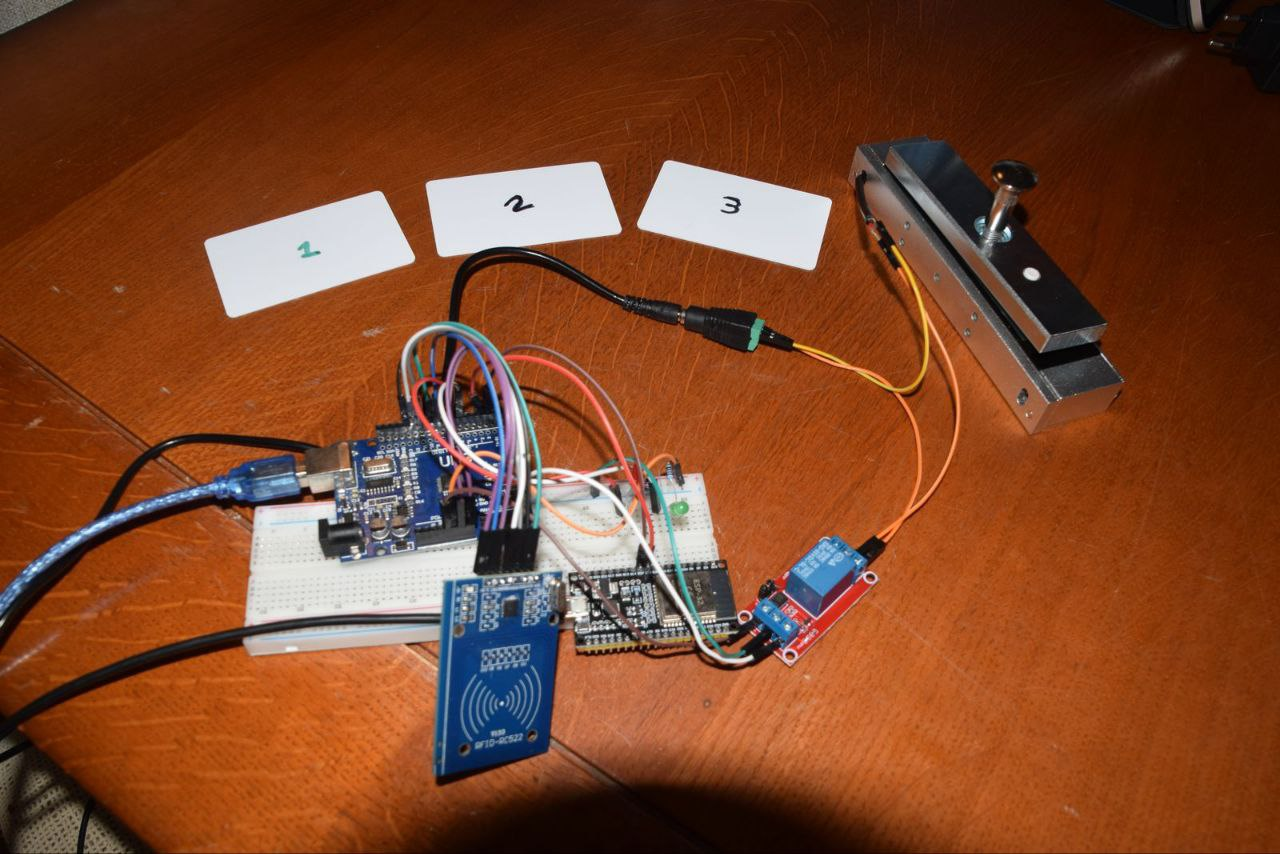
\includegraphics[width=0.8\textwidth]{imaxes/NACU} % Inserta aquí la imagen real si la tienes
	\caption{NACU and Test Cards. From left to right, the Arduino Uno, MFRC522, ESP32 and magnetic lock can be seen. Also, the three cards at the back are the ones used to test the system.}
	\label{fig:nacu_hardware}
\end{figure}

\section{Access Control Management Server (ACMS)}
\label{sec:acms}

As a result of the incremental development of ACMS, a complete system with the following functional capabilities was obtained:
\begin{itemize}
	\item User and role management: adding and deleting users with permissions assignment.
	\item Credential control: loading and protection of master keys in the simulated HSM and AppKey derivation.
	\item Access validation: reception of NACU requests, UID and time window checking, and allow or deny access control.
	\item Real-time auditing: detailed log of each entry attempt.
	\item Alert system: immediate email notification in case of unauthorized access.
	\item Administrative interface: web views to view access logs, manage schedules, review and revoke credentials.
\end{itemize}

The ACMS, \ref{sec:ACMS}, was implemented in Django following an incremental methodology. In the first phase the REST API base was created, and in the following phases security, management and presentation functionalities were added until completing a server capable of processing all NACU access trial requests. The architecture, shown in Figure~\ref{fig:acms_architecture}, combines a Django server over HTTPS/TLS, with its own default model database, with a software Hardware Security Module (HSM) implementation (SoftHSM/PKCS\#11) to protect cryptographic keys.

\begin{figure}[h]
	\centering
	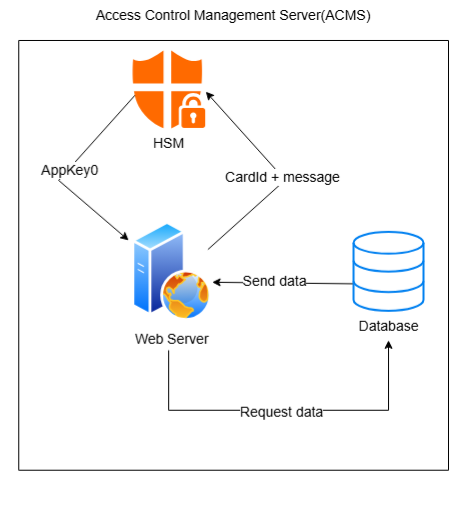
\includegraphics[width=0.8\textwidth]{imaxes/ACMS} % Inserta aquí la imagen real si la tienes
	\caption{ACMS Architecture Scheme including HSM, the web server and the default Django model database}
	\label{fig:acms_architecture}
\end{figure}

This architecture is able to perform the following protocols in order to process NACU requests:
\begin{itemize}
	\item Key derivation via HMAC-SHA256 in the HSM, so that the NACU can request the key needed for reading the card UID and it can be successfully obtained without storing it in a vulnerable database or exposing the master key.
	\item NFC personal UID validation on ACMS, managing time-based access control.
\end{itemize}

Also, an administration interface was defined using the default views offered by Django, including a login view (Figure~\ref{fig:login_view}) and an administration panel for data modeling. In addition, a log list view (Figure~\ref{fig:log_list_view}) was created for the administrator to be able to check all the access attempts into the physical facility that the access control system is protecting. By displaying both successful and failed attempts, this view gives administrators a clear audit trail to spot unusual patterns, investigate security incidents, verify policy compliance and fine-tune access rules over time.

\begin{figure}[h]
	\centering
	\includegraphics[width=\textwidth]{imaxes/login} 
	\caption{Administration Default Login system}
	\label{fig:login_view}
\end{figure}

\begin{figure}[H]
	\centering
	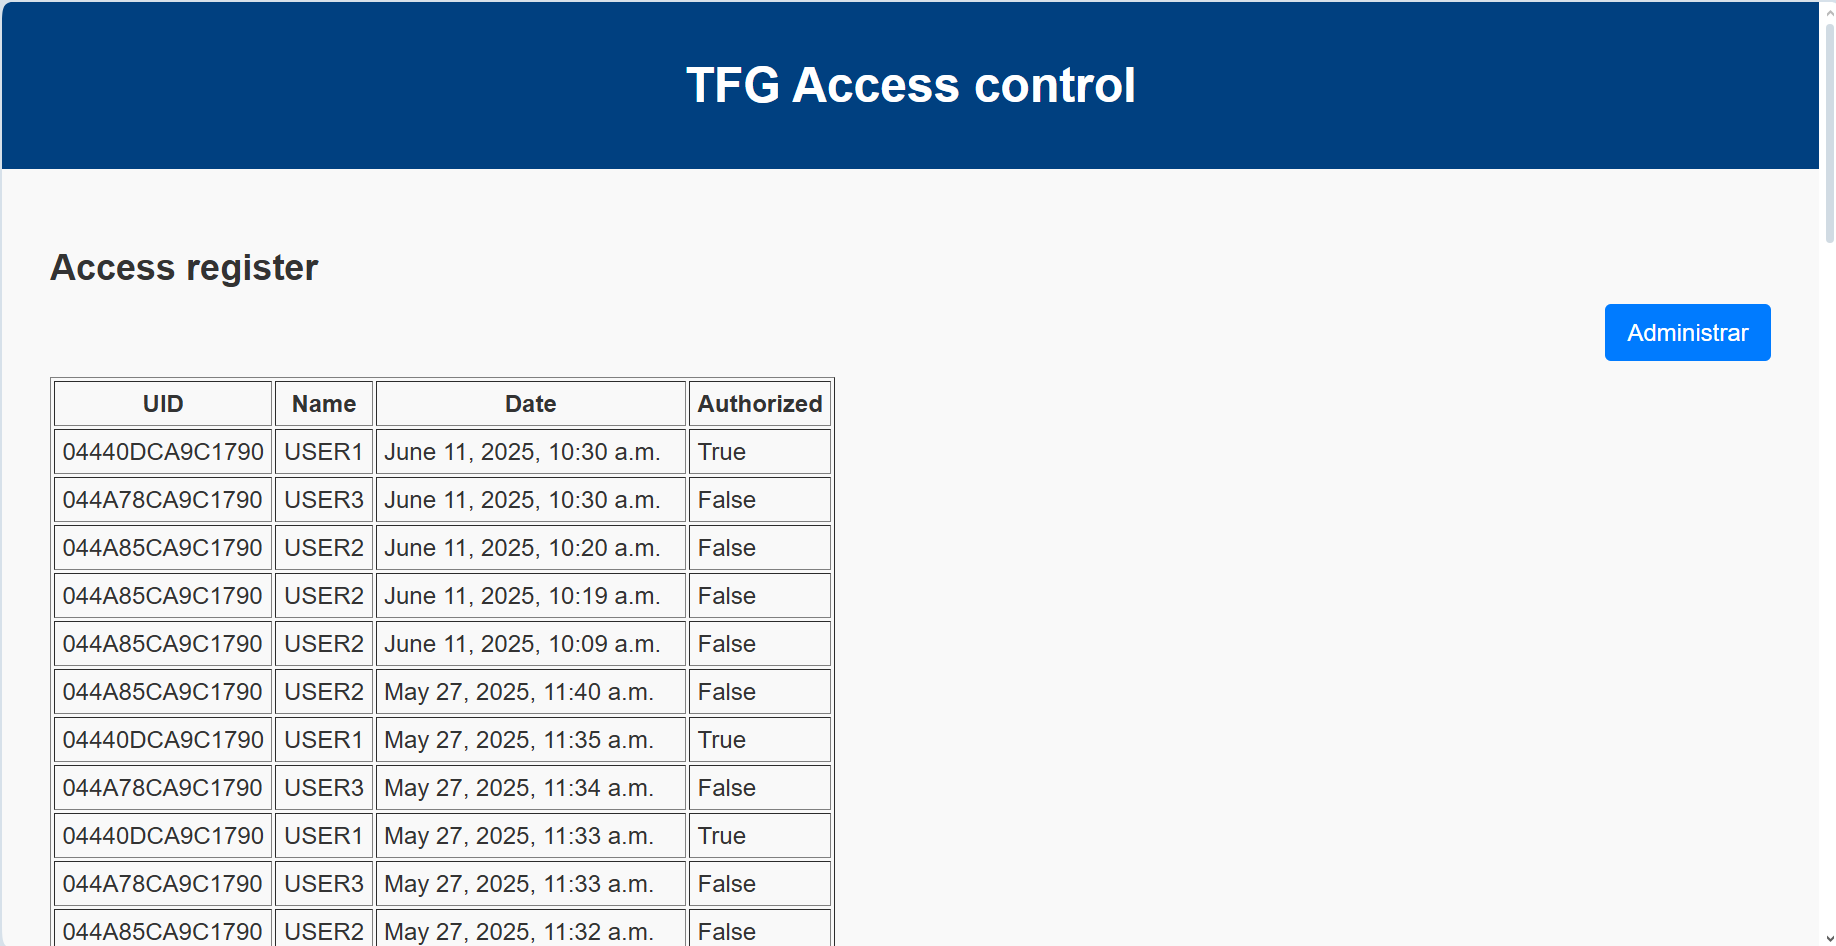
\includegraphics[width=\textwidth]{imaxes/loglist} % Inserta aquí la imagen real si la tienes
	\caption{Log List Administration View}
	\label{fig:log_list_view}
\end{figure}

\clearpage

\subsection{Defined Endpoints}
The endpoints defined for this project are presented below. The ACMS code is completely open-source and is organized in a modular way, so that new functionalities can be easily incorporated on this already implemented base.

\begin{table}[H]

	\begin{tabular}{|l|l|p{2.5cm}|p{2.5cm}|}
		\hline
		\textbf{Endpoint} & \textbf{Method} & \textbf{Request payload} & \textbf{Response Payload} \\ \hline
		/submit\_uid/ & GET & uid (hexadecimal string, required) & JSON \{ message, uid, timestamp, authorized[, error] \} \\ \hline
		/authenticate\_uid/ & GET & uid (hexadecimal string, required) & Redirect to log\_list view (HTML with log list) \\ \hline
		/log\_list/ & GET & --- & HTML rendering of core/log\_list.html with logs \\ \hline
		/compute\_appkey0/ & GET & cardid (hex), msg (string) & JSON (pure) with hex string of 32 chars or error JSON \\ \hline
	\end{tabular}
	\caption{ACMS Endpoints Overview}
	\label{tab:endpoints}
\end{table}

\section{Key Management and Security System}
In this system, a software-based Hardware Security Module (SoftHSM) was built and integrated into the ACMS authentication server to safeguard all critical cryptographic material. Rather than relying on Django’s default key handling, SoftHSM, a software HSM implementation (PKCS\#11-compatible), was implemented to store the Master Key securely and derive per-card AppKey0 values via HMAC-SHA256. An ACMS endpoint receives a cardId and a msg, forwards them to the HSM for secure key derivation, and returns only the resulting AppKey0, ensuring that neither the Master Key nor any intermediate secrets ever leave the protected HSM environment. This custom HSM integration follows the key management architecture laid out in \ref{subsec:keymanagement} (Figure~\ref{fig:key_management}).

\begin{figure}[h]
	\centering
	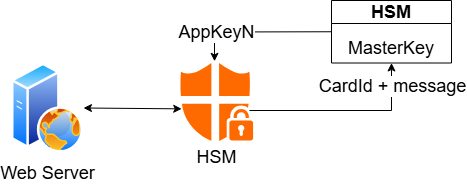
\includegraphics[width=0.7\textwidth]{imaxes/KEY_MANA} % Inserta aquí la imagen real si la tienes
	\caption{Key Management System in the HSM}
	\label{fig:key_management}
\end{figure}

For protecting the master key:
\begin{itemize}
	\item A token is initialized using SoftHSM, creating a secure disk slot protected by an administrator PIN and user PIN.
	\item The Master Key is loaded into the token, making it impossible to retrieve in clear text.
\end{itemize}

Then, the endpoint /compute\_appkey0/ was created to derive AppKey0 via HMAC-SHA256 from a cardId and a msg, using the Master Key without ever exposing it. Protecting the Master Key is critical; its compromise would endanger the confidentiality of every derived key and, ultimately, the security of the entire system.

\section{Access Control System Secure Communications}
To ensure the confidentiality and integrity of communications between the NACUs and the ACMS server, in the third iteration of the incremental development of it (\ref{subsec:https}), the channel was changed from HTTP to HTTPS/TLS in the development environment. Django-sslserver was integrated to enable TLS on the Django server and Mkcert was used to generate a local Certificate Authority that issues X.509 certificates trusted by the operating system and browsers. On the Wi-Fi module, the WiFiClientSecure library was used to establish TLS connections, configured to accept Mkcert's self-signed certificates. Thanks to this setup, all REST requests are end-to-end encrypted, ensuring that both credentials and sensitive data travel securely without validation errors or local security warnings.

\section{Role-based Access Control Management}
As explained in \ref{subsec:roles}, the system was extended with basic profile-based access control and multi-reader identification. This feature allows administrators to tailor entry permissions per user group; granting, for example, employees access to internal offices while restricting guests to reception areas, thus managing who can open which doors in a multi-reader deployment simply by assigning roles.

A new Role model was linked one-to-one with HSMData, allowing administrators in the Django panel to assign roles (e.g., “admin”, “employee”, “guest”), as shown in Figure~\ref{fig:role_management}, directly when creating or editing users. To distinguish between multiple NACU units, a helper was implemented in views.py to parse the reader ID messages of the form “GETUIDN” at the /compute\_appkey0/ endpoint. This process enables the log to capture both the user’s role and the originating reader, demonstrating how future production logic could enforce fine-grained rules (for example, “only admins may use reader 2”). In this prototype phase, recording these values suffices to validate the feasibility of integrating roles and reader detection into the authorization workflow.

\begin{figure}[h]
	\centering
	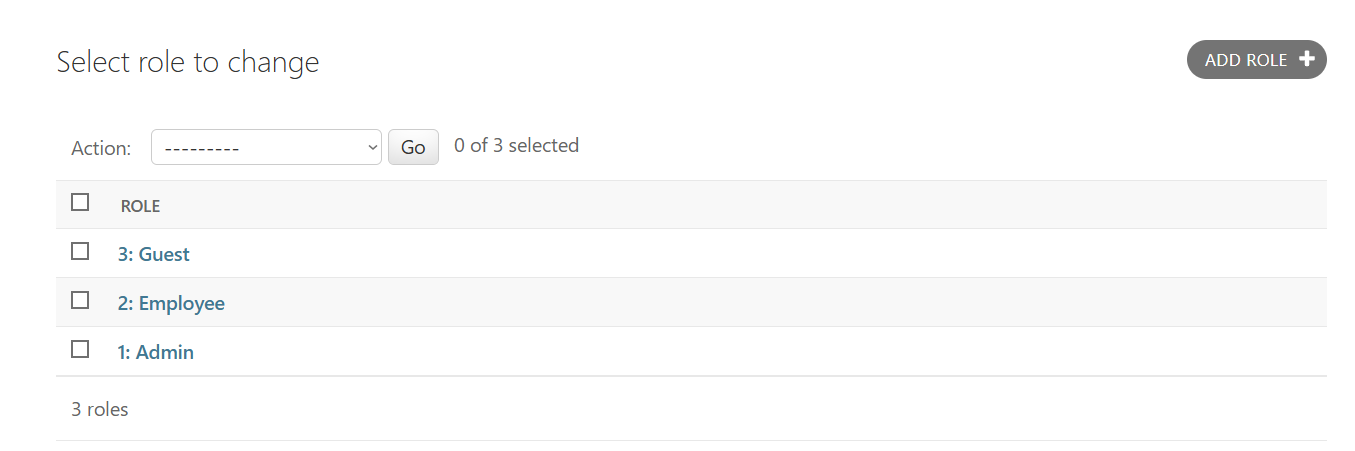
\includegraphics[width=0.7\textwidth]{imaxes/Roles} % Inserta aquí la imagen real si la tienes
	\caption{Role Management view}
	\label{fig:role_management}
\end{figure}

\section{Real-time Unauthorized Access Attempt Alert System}
Real-time email notifications enable a company to detect and respond immediately to security incidents, reducing the window of vulnerability, improving compliance with audit requirements, and minimizing the risk of unauthorized entry. In this forth iteration, as explained in \ref{subsec:email}, immediate email notifications for unauthorized access attempts were integrated directly into the /submit\_uid/ view. Using Django’s built-in SMTP backend, configured to work with TLS and STARTTLS on port 587, the system encrypts credentials and message content end-to-end. Also, to balance immediacy and reliability, alerts are sent synchronously, ensuring the administrator is notified as soon as an incident is logged, while the \texttt{fail\_silently} option is set to True in order to prevent SMTP errors from disrupting the access-control flow. This prototype demonstrates a robust, low-overhead mechanism for real-time monitoring of critical events.

\begin{figure}[h]
	\centering
	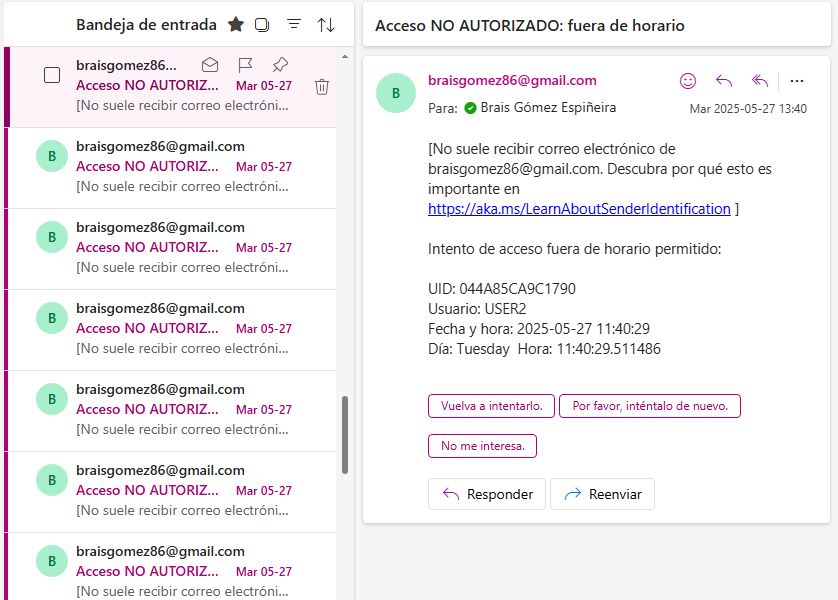
\includegraphics[width=0.7\textwidth]{imaxes/MAIL} % Inserta aquí la imagen real si la tienes
	\caption{Unauthorized Mails Example}
	\label{fig:unauthorized_mail}
\end{figure}
